\documentclass[12pt]{article}

\usepackage[left=1.5in,right=1.5in,top=1.5in,bottom=1.5in]{geometry}
\usepackage{fancyhdr}
\usepackage{graphicx}
\usepackage[hyperfootnotes=false]{hyperref}
\usepackage{subcaption}
\usepackage[utf8]{inputenc}

\pagestyle{fancy}
\fancyhf{}
\lhead{\small Honeycomb: An Ecosystem Hub for Decentralized Oracle Networks}
%\rhead{\vspace{-1cm} 
\includegraphics[width=1cm]{Figures/honeycomb_solo}}
\fancyfoot[C]{\thepage}

\begin{document}

\pagenumbering{gobble} 
\title{\vspace{-2cm} 
\includegraphics[height=3cm]{Figures/honeycomb_solo} \\\vspace{2cm} \textbf{\Large Honeycomb: An Ecosystem Hub \\ for Decentralized Oracle Networks}}
	
\author{Burak Benligiray, Dave Connor, Adam Tate, Heikki Vänttinen}

\date{\href{https://honeycomb.market}{honeycomb.market}\\ \medskip 4~February~2019, v1.0}
	
\maketitle

\begin{abstract}
Smart contracts require oracles to access real-world data and perform meaningful actions.
Chainlink is a trustless oracle network aiming to become the industry standard.
Although Chainlink is designed to benefit all participants in its ecosystem greatly once adoption takes place, reaching that point is not a trivial problem.
CLC Group aims to assist in bootstrapping the Chainlink ecosystem by facilitating mutually beneficial partnerships through ecosystem-scale services.
The first of these services is Honeycomb, an API marketplace website that is going to serve external adapters to Chainlink node operators under a software-as-a-service model.
Nodary, the first Chainlink oracle certification service, validates oracle identities as not being able to perform Sybil attacks.
Finally, a free-to-use listing service is proposed to make sure that smart contract developers can find Nodarized oracles that serve Honeycomb APIs.
The combination of these services is planned to create a network effect that positions Honeycomb as an ecosystem hub.
{\let\thefootnote\relax\footnote{{We thank Thomas Hodges and Jonny Huxtable for reviewing an earlier version of this paper.}}}
\end{abstract}

\newpage
\pagenumbering{arabic}
\setcounter{page}{1}


%~~~~~~~~~~~~~~~~~~~~~~~~~~~~~~~~~~~~~~~~~~~~~~~~~~~~~~~~~~~~~~~~~~~~~~~~~~~~~~~~~~~~~~
\section{Introduction}
\label{sec:introduction}

``Business is done at the speed of trust."
Although this saying is traditionally used to emphasize the importance of trust, it has an obscure implication: The need for trust is an absolute limit for all business transactions.
Consequently, eliminating this need would result in an unprecedented economic expansion.
Smart contracts are software that are designed to execute transactions only if all parties fulfill their obligations~\cite{Szabo:1994}.
In other words, they eliminate the need for mutual trust between parties or a trusted intermediary.
As a result, they are expected to transform how business is done~\cite{Chamber:2016}.

According to Capgemini's report~\cite{Capgemini:2016}, by reducing the settlement period for leveraged loans with smart contracts, a loan volume growth of \$149 billion can be achieved.
In the same report, it has been estimated that up to \$11 billion savings can be generated in the US and Europe by improving the efficiency of mortgage processes through smart contracts.
Across geographies, sectors and use-cases, the potential value that can be generated by adopting smart contracts is immense.
Gartner forecasts blockchain-based technologies to create global business value of over \$176 billion by 2025, and \$3.1 trillion by 2030~\cite{Gartner:2017}.

Despite its potential, Ethereum~\cite{Buterin:2014}, a public smart contract platform that has been online since 2015, has not yet been utilized for commercial activity to a revolutionary degree~\cite{Bartoletti:2017}.
This can mainly be attributed to what is referred to as the oracle problem~\cite{Barr:2015}, which expresses the difficulty of satisfactorily determining if an obligation is fulfilled or a condition is met in the context of a smart contract.
Ethereum's scope does not include a built-in trustless solution to the oracle problem, as per their motto: ``We have no features"~\cite{Ethereum:2014}.
Instead, the development of trustless oracles is delegated to third parties.
A trustless oracle network has yet to be implemented, which has prevented Ethereum from providing end-to-end trustlessness, and thus being widely adopted for commercial applications.

Chainlink is a promising decentralized oracle network infrastructure~\cite{Ellis:2017}. Its planned features are:
\begin{itemize}
	\item Aggregation from multiple oracle nodes to provide trustlessness;
	\item Cross-chain functionality, meaning that it can serve any smart contract platform, including private/permissioned blockchains;
	\item Third party reputation and certification support;
	\item Optionally letting the requester enforce the use of trusted execution environments (e.g., Intel SGX~\cite{Costan:2016}), which ensures the integrity and privacy of the operation delegated to oracle nodes.
\end{itemize}
The combination of these features sets Chainlink to become the backbone of the smart contract economy.
However, similar to all attempts at establishing infrastructure, technology is only half of the question, the other being the adoption process.

The Chainlink ecosystem is going to consist of \textbf{API providers} (existing businesses), Chainlink \textbf{node operators} and \textbf{smart contract developers}.
When adoption is complete, each participant is going to be entangled in a complex yet sustainable network of mutual interest.
However, the status quo encourages sluggishness in adoption. Each group would rather have the other two adopt Chainlink before them, resulting in a gridlock.
As a neutral third party, CLC Group aims to catalyze the adoption process.
Through our services, we are going to cultivate immediate mutual interest between parties, and thus stimulate simultaneous adoption.
With each bridge built between the members of the ecosystem, we aim to bring a smart contract-run economy one step closer.

We have detected the most immediate deficiencies in the ecosystem, and designed services that are both going to remedy these and reinforce each other.
\begin{itemize}
	\item There is no venue where API providers can reach node operators to serve their data, and node operators can find APIs to subscribe to.
	Accordingly, our first course of action is to launch \textbf{Honeycomb}, a marketplace website where we are going to bring API providers and node operators together (see Section~\ref{sec:honeycombapimarketplace}).
	\item The node operators currently cannot prove their trustworthiness to smart contract developers.
	As a solution, we are going to set up \textbf{Nodary}, the first Chainlink oracle certification service (see Section~\ref{sec:nodary}).
	By getting Nodarized, node operators prove that they are unable to perform Sybil attacks, which require running multiple oracles as a single operator.
	\item Smart contract developers are going to be looking for trustworthy oracles with good access to data.
	We are going to maintain a listing service that smart contract developers can use to access a list of Nodarized oracles that serve Honeycomb APIs (see Section~\ref{sec:honeycombasanecosystemhub}).
	Getting oracles listed on this service and accessing listed oracles will be free of charge.
\end{itemize}
By serving Nodary and a free listing service over the Honeycomb marketplace website, we are aiming to create a center of attraction for the whole ecosystem that is going to foster mutually beneficial partnerships, while positioning Honeycomb to become an ecosystem hub.


%~~~~~~~~~~~~~~~~~~~~~~~~~~~~~~~~~~~~~~~~~~~~~~~~~~~~~~~~~~~~~~~~~~~~~~~~~~~~~~~~~~~~~~
\section{Chainlink}
\label{sec:chainlink}

An API (application programming interface) is a protocol that allows software to use the functions of another software.
For example, financial asset management software would periodically use the APIs of exchanges to fetch price data and send trading orders over the Internet to re-balance the portfolio.
An API can be implemented to retrieve any data or trigger any event remotely.
Therefore, enabling smart contracts to use APIs would allow them to be used in nearly all potential applications.
Smart contracts cannot use APIs directly because they can only operate on the blockchain they reside in, but cannot communicate over the Internet.
To be able to communicate with APIs over the Internet, smart contracts need intermediaries that can operate both on the respective blockchain and the Internet, called oracles.

\begin{figure}
	\centering
	\begin{subfigure}{.5\textwidth}
		\centering
		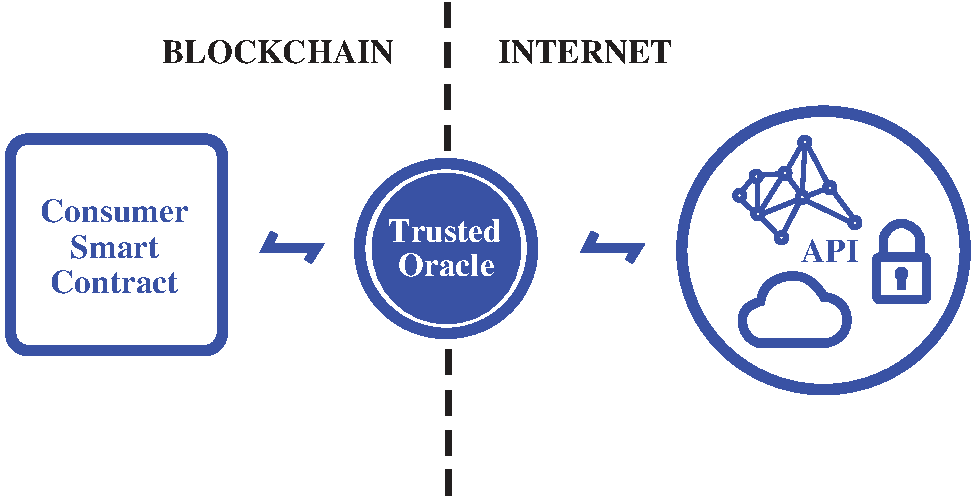
\includegraphics[height=.45\linewidth]{Figures/oracle1}
		\caption{Trusted oracle}
		\label{fig:oracleproblem1}
	\end{subfigure}%
	\begin{subfigure}{.5\textwidth}
		\centering
		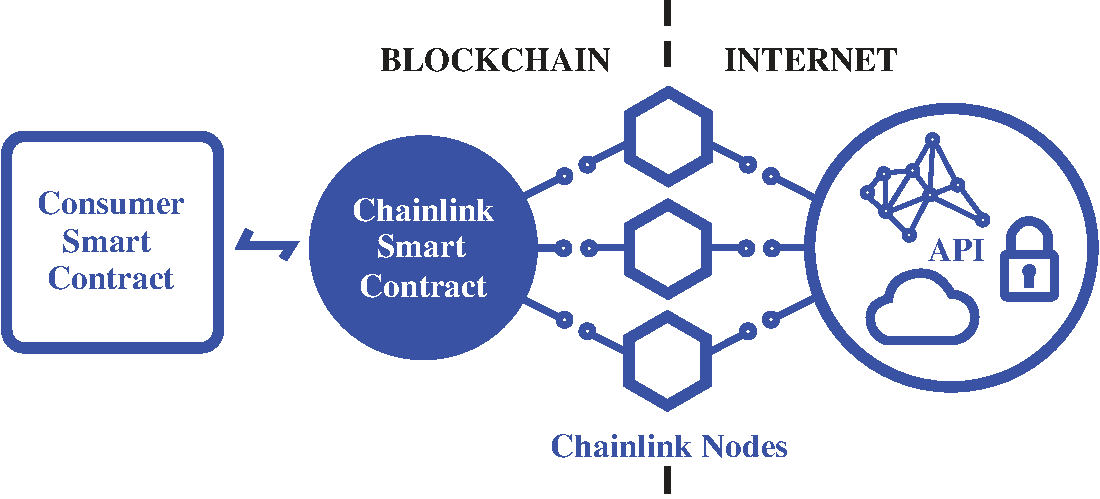
\includegraphics[height=.45\linewidth]{Figures/oracle2}
		\caption{Decentralized oracle network}
		\label{fig:oracleproblem2}
	\end{subfigure}
	\caption{Two approaches to the oracle problem:
		(a) In the traditional approach, a single trusted oracle mediates between the requester smart contract and the API.
		(b) With the decentralized oracle network, multiple oracles interact with the API independently, the results are aggregated by a smart contract and passed to the consumer smart contract.}
	\label{fig:oracleproblem}
\end{figure}

Let us start by describing the traditional approach in interfacing a smart contract with an API (see Figure~\ref{fig:oracleproblem1}).
The requesting smart contract initiates the process by writing the details of its request on the blockchain.
An oracle software run on a single machine reads this information from the blockchain and calls the API accordingly.
Then, the oracle writes the response back to the blockchain for the smart contract to read.
This approach is seriously questionable, because it requires the oracle to be trusted.
In the case that the operator of the oracle is malicious or the machine that the oracle software runs on is compromised, the outcome of the smart contract can be manipulated.
Such a risk defeats the entire purpose of using smart contracts, which is to transact reliably without any of the involved parties having to trust a single entity.

Chainlink uses a decentralized oracle network (see Figure~\ref{fig:oracleproblem2}).
The essence of this approach is to ask multiple Chainlink nodes to fulfill the same request, reduce their report into one and return it to the requesting smart contract.
Each oracle node is rewarded with LINK tokens by the requesting smart contract if its answer agrees with the other nodes’ answers.
If a node’s answer is conflicting with the general consensus, it is penalized by the amount of LINK tokens staked by that node as collateral.
The resulting system ensures that the requests are fulfilled correctly without having to rely on a single individual, granted that the nodes are operated by independent and competing actors.
In Section~\ref{sec:nodary}, we are going to describe Nodary, a service that ensures that these assumptions are satisfied.

In the remainder of this section, we are going to give simplified explanations to some concepts that are related to the services that we are planning to offer.
Refer to the Chainlink white paper~\cite{Ellis:2017} for more details as needed.

%~~~~~~~~~~~~~~~~~~~~~~~~~~~~~~~~~~~~~~~~~~~~~~~~~~~~~~~~~~~~~~~~~~~~~~~~~~~~~~~~~~~~~~
\subsection{External adapters}
\label{sec:externaladapters}

APIs that provide high value data, critical functionality or accessibility guarantees are typically authenticated.
This means for the API to only answer authorized users (e.g., paid subscribers), and this is usually verified by the API key provided by the user.
The consumer smart contract announces the job details regarding its request publicly.
The API key cannot be a part of this announcement, because it needs to be kept secret from the public.

\begin{figure}
	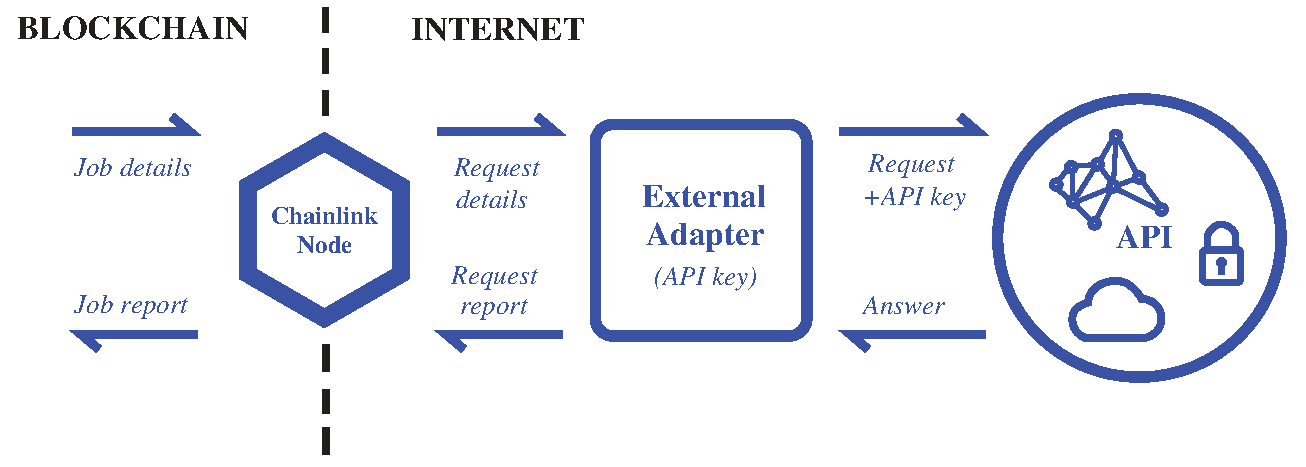
\includegraphics[width=\textwidth]{Figures/externaladapter}
	\caption{Using an external adapter to pass the API key to the API provider.}
	\label{fig:externaladapter}
\end{figure}

Chainlink has solved this problem through a concept called external adapter, which is third party software that is used in combination with core Chainlink node software.
See Figure~\ref{fig:externaladapter} for an illustration of its function.
The process starts with the Chainlink node receiving the details of a job from the Chainlink smart contract.
This job is typically composed of multiple steps, one being a request to an API.
The Chainlink node passes the details of the request to be made to the external adapter.
The external adapter combines the request details and the API key, and makes the request.
Then, the results are passed back to the Chainlink smart contract.
Note that the API key is not made public on the blockchain, and neither does the Chainlink node software handle it.
    
Since API design is not strictly standardized, a special external adapter has to be developed to interface with each individual API, which creates a barrier to entry for APIs to become available on the Chainlink network.
Furthermore, it is not clear whose responsibility it is between the API provider and the node operators to develop this external adapter, which can result in a gridlock where neither party wants to allocate resources to build it.

There are two configurations for operating an external adapter.
In the first configuration, the external adapter runs on the same machine as the Chainlink node.
In this scenario, the node operator is going to download and run an external adapter on their node machine for each authenticated API they want to serve.
In the alternative configuration, the node operator connects their node to a set of remote external adapters.
We are going to discuss the advantages of this second approach in Section~\ref{sec:externaladaptersassaas} under the title ``External adapters as SaaS".

%~~~~~~~~~~~~~~~~~~~~~~~~~~~~~~~~~~~~~~~~~~~~~~~~~~~~~~~~~~~~~~~~~~~~~~~~~~~~~~~~~~~~~~
\subsection{Listing services}
\label{sec:listingservices}

There are two ways for a requesting smart contract to determine the nodes that are going to serve it (see Figure~\ref{fig:oracleproblem2}).
In the first method, the requester finds a group of nodes that satisfy its requirements and sends them proposals for the related job.
Once all nodes agree to the job, the finalized service level agreement gets pushed to the blockchain.
Alternatively, an order-matching smart contract acts as a public job board that nodes watch to apply for jobs that they are qualified for.

To be able to use the first method, the smart contract developer needs to be able to access a list of oracles.
Furthermore, this list should be filterable according to the requester’s requirements (e.g., reputation score, certification status, price).~This function of providing requesters with a list of eligible oracles is the main feature of a listing service.
We will introduce a listing service maintained by CLC Group in Section~\ref{sec:honeycombasanecosystemhub}.


%~~~~~~~~~~~~~~~~~~~~~~~~~~~~~~~~~~~~~~~~~~~~~~~~~~~~~~~~~~~~~~~~~~~~~~~~~~~~~~~~~~~~~~
\section{Chainlink Ecosystem}
\label{sec:chainlinkecosystem}

The Chainlink ecosystem is composed of three groups of actors:
\begin{itemize}
	\item \textbf{API providers} run APIs that can be triggered over the Internet to execute specific actions.
	\item \textbf{Node operators} run Chainlink nodes that call APIs as requested by smart contracts.
	\item \textbf{Smart contract developers} develop smart contracts that need Chainlink nodes to call APIs.
\end{itemize}

\begin{figure}
	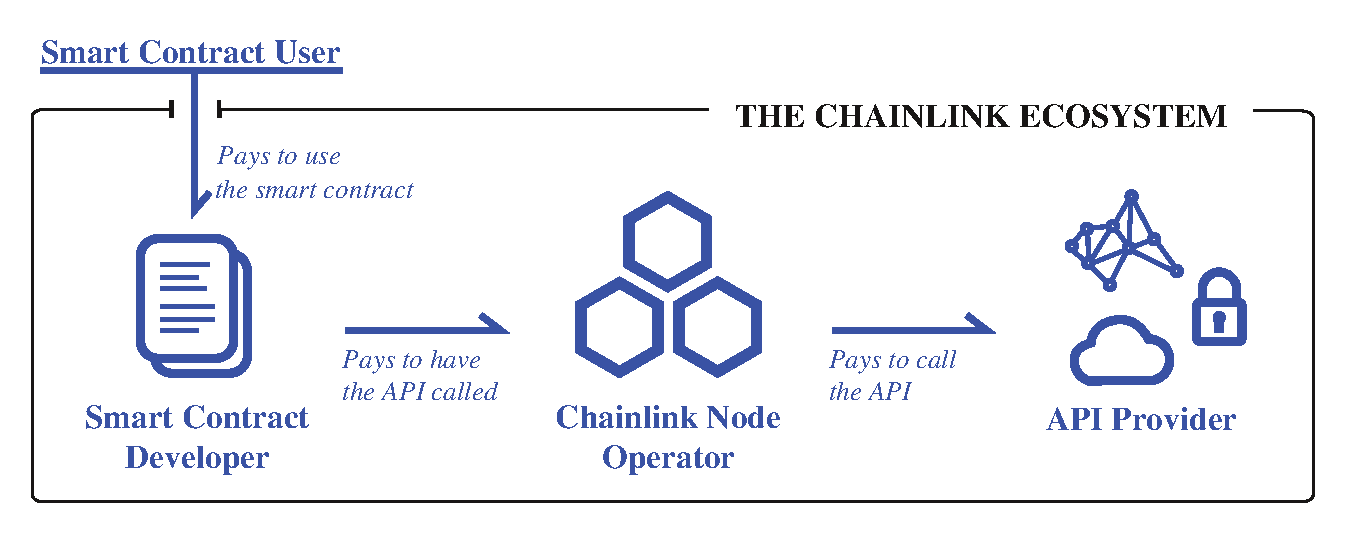
\includegraphics[width=\textwidth]{Figures/cashflow}
	\caption{Three groups constituting the Chainlink ecosystem and the flow of funds between them.}
	\label{fig:cashflow}
\end{figure}

To understand the relationship between these groups, let us start by investigating the flow of funds.
As can be seen on Figure~\ref{fig:cashflow}, the system is not self-contained, but fed by the smart contract users.
These users typically pay a convenience fee to use the smart contract, which is the main source of income of the smart contract developers.
To have requests made to an API, the smart contract developer pays Chainlink node operators.
If the API to be called is not free, the node operators pay the API provider.
In a way, the revenue trickles down from smart contract developers, to node operators, to API providers.
In this aspect, the three groups share a single pie, and thus are incentivized to minimize each other’s shares.
It is common for cartels to be formed in unregulated markets to achieve such ends by boycotting, fixing prices and rigging bids.

The alternative of economic collusion is a market where API providers, node operators and smart contract developers compete among their respective groups.
Price competition is healthy, as it fosters efficiency, decreases smart contract operation costs, and as a result, supports smart contract adoption.
However, it would be overly optimistic to expect this competition to be limited to pricing.
The actors are going to be incentivized to withhold helpful information as trade secrets, and may go as far as targeting direct competitors.
For example, a node operator who has developed an external adapter for an API may rather not distribute it to other node operators for the sake of having monopoly power.

The ecosystem is wildly heterogeneous with asymmetrical relationships, and both the groups and group members are in direct competition.
The community cannot be expected to spontaneously cooperate to achieve large scale adoption, which is the state where there is a wide variety of smart contracts, nodes and APIs to facilitate free-market conditions.

\subsection{CLC Group}
\label{sec:clcgroup}

CLC Group was founded to support the growth of the Chainlink ecosystem through its lifetime.
In the initial stages, the focus is going to be on getting the newly implemented functions to start being utilized, and getting outside players to engage with the Chainlink network.
As the network matures, we are going to focus on streamlining our products, and implementing new use-cases for Chainlink and smart contracts in general.

Among the teams that are working with Chainlink, CLC Group possesses a unique quality.
It is not an API provider, a node operator or a smart contract developer.
As a result, it is not in inherent conflict of interest with any of the players within the ecosystem.
This neutrality allows CLC Group to be able to operate under a business model that benefits all participants without bias.

CLC Group aims to build a hub in the Chainlink ecosystem that facilitates mutually beneficial partnerships between groups through a variety of services.
These include small-scale consultancy services that connect a particular group of players, and highly scalable services that target the entire ecosystem at once.
In the following sections, we are going to introduce some of these ecosystem-scale services.


%~~~~~~~~~~~~~~~~~~~~~~~~~~~~~~~~~~~~~~~~~~~~~~~~~~~~~~~~~~~~~~~~~~~~~~~~~~~~~~~~~~~~~~
\section{Honeycomb as an Ecosystem Hub}
\label{sec:honeycombasanecosystemhub}

\begin{figure}
	\centering
	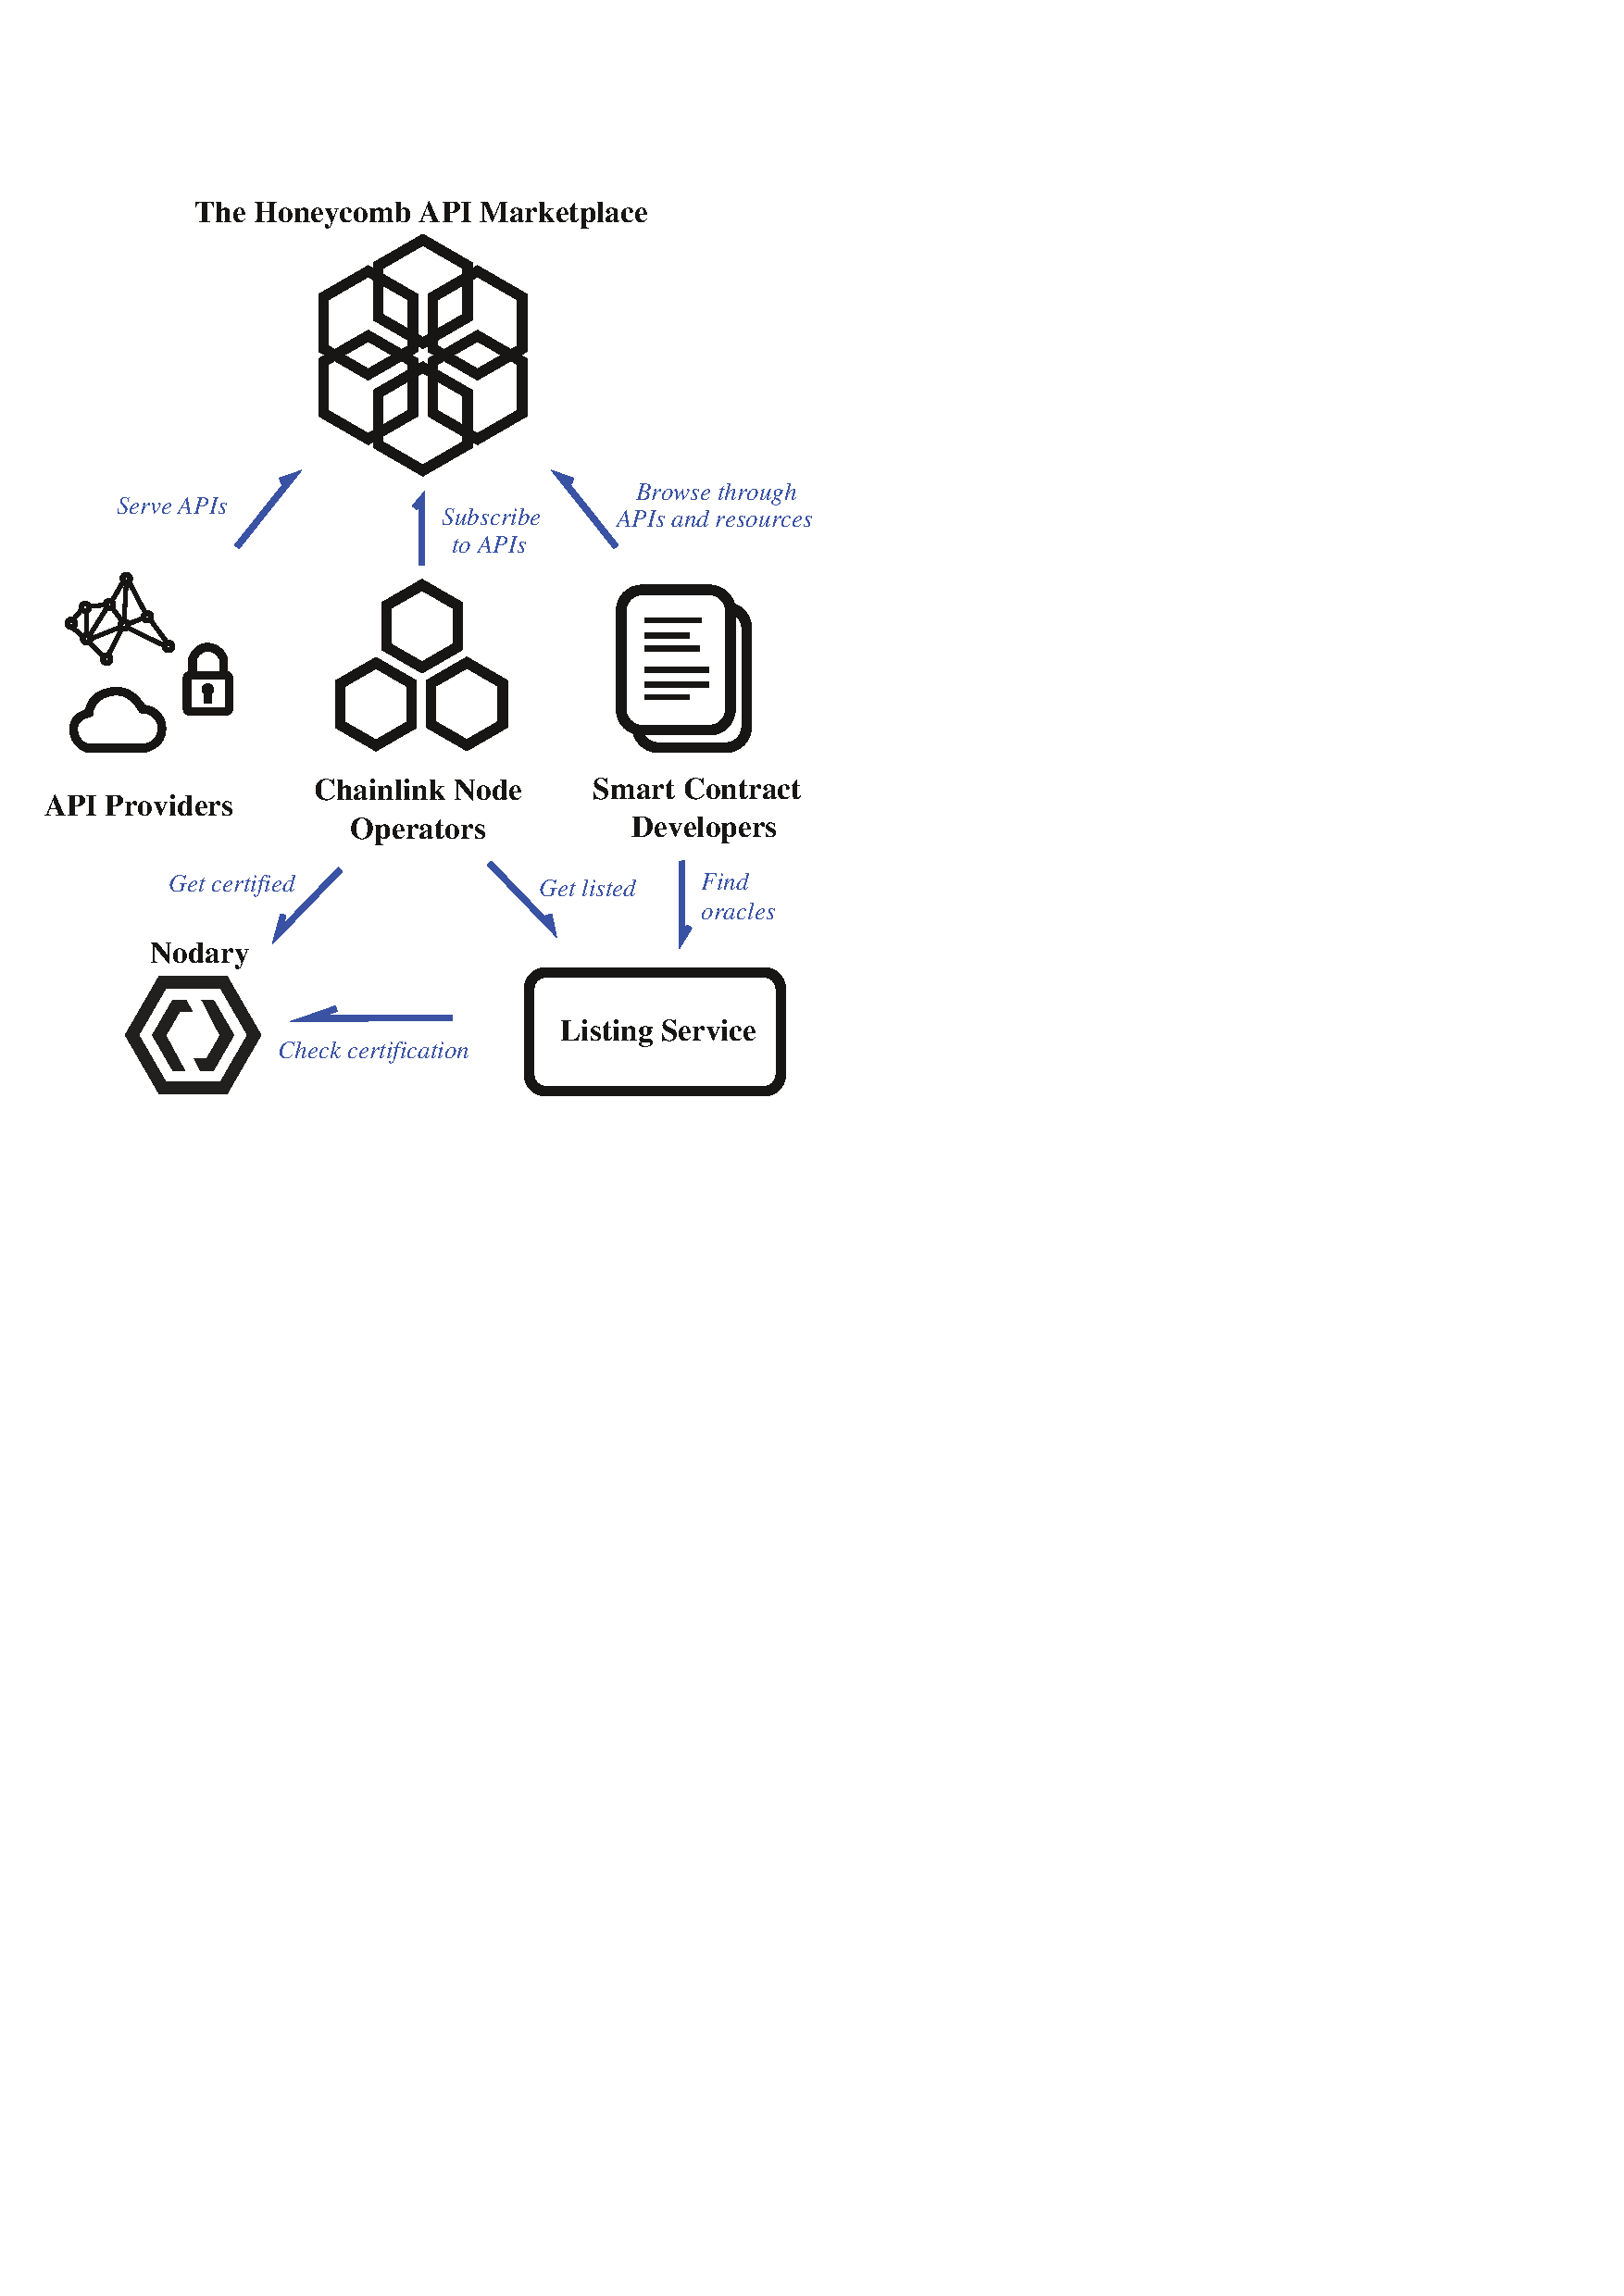
\includegraphics[width=0.5\textwidth]{Figures/ecosystem}
	\caption{The Honeycomb marketplace, listing service, and Nodary, a certification service, as connections that are going to make Honeycomb into an ecosystem hub.}
	\label{fig:ecosystem}
\end{figure}

We aim to build an ecosystem hub where API providers, node operators and smart contract developers will come together and form mutually beneficial partnerships.
To be able to achieve this, we will provide services that meet the needs of each group.
Namely, these services will be the Honeycomb API marketplace, the Honeycomb listing service and Nodary, an oracle certification service.
See Figure~\ref{fig:ecosystem} for an overview of how these services connect the ecosystem players to Honeycomb and each other.

At its core, Honeycomb is a marketplace website for API providers to offer their services to node operators, and thus connects these groups.
In addition to this, we expect the smart contract developers to search through the API listings to find data sources to be utilized in their smart contracts.
The second service we are going to provide over Honeycomb is Nodary, an oracle certification service, which is going to create additional incentive for node operators to use Honeycomb.
We are going to reinforce this synergy by allowing Nodarized node operators to access all external adapters on the Honeycomb marketplace for free.
This strategy also guarantees all Honeycomb APIs to be accessible at all times over the Nodarized oracles.

As described in Section~\ref{sec:listingservices}, listing services are critical for smart contract developers to find oracles that meet their requirements.
This fits our vision for Honeycomb as a connector between the groups in the ecosystem perfectly, which is why we have also decided to operate a listing service integrated to it.
Our aim is for this service to be free for both node operators and smart contract developers to assist the growth of the Chainlink network, and have more players use Honeycomb.
However, our priority during the initial implementation is going to be Nodarized node operators serving Honeycomb APIs.
Once the listing service is open to all node operators, smart contract developers are still going to be able to filter oracles by Nodarization status.

The importance of smart contract developers to the Chainlink ecosystem cannot be overemphasized.
Referring back to Figure~\ref{fig:cashflow}, smart contracts that create value for their users are vital for the ecosystem to thrive.
For this reason, we see smart contract developer engagement with Honeycomb to be crucial for its success, and are going to increase this through the following means:
\begin{itemize}
	\item Informational resources that are going to enable smart contract developers to take advantage of the functionalities that a Honeycomb-powered oracle network provides;
	\item A directory of public and authenticated APIs, associated jobs and smart contracts, maintained by the community under a wiki format;
	\item Hackathons and competitions to implement smart contracts that utilize Honeycomb APIs to increase awareness of Honeycomb and its APIs, and assist in coming up with novel use-cases for smart contracts.
\end{itemize}
In addition to these, the APIs that are in high demand by the smart contract developers are going to be our number one priority to have on the Honeycomb marketplace.


%~~~~~~~~~~~~~~~~~~~~~~~~~~~~~~~~~~~~~~~~~~~~~~~~~~~~~~~~~~~~~~~~~~~~~~~~~~~~~~~~~~~~~~
\section{Honeycomb API Marketplace}
\label{sec:honeycombapimarketplace}

To have an authenticated API available on the Chainlink network, node operators have to subscribe to the said API for a fee and intermediate requests to it.
To facilitate this happening at scale, we propose the Honeycomb marketplace, a website for API providers to offer their services to node operators. Its main features are as follow:
\begin{itemize}
	\item A catalog of authenticated APIs, acting as a venue for API providers to make their product visible to node operators and smart contract developers;
	\item External adapters under SaaS model, developed, operated and maintained by CLC Group, designed to be user-friendly, secure, highly accessible and scalable;
	\item Per-call pricing for both node operators and API providers;
	\item Option to pay in cryptocurrency for node operators;
	\item Allows node operators to easily manage their API portfolio and payments through a graphical user interface.
\end{itemize}

%~~~~~~~~~~~~~~~~~~~~~~~~~~~~~~~~~~~~~~~~~~~~~~~~~~~~~~~~~~~~~~~~~~~~~~~~~~~~~~~~~~~~~~
\subsection{External adapters as SaaS}
\label{sec:externaladaptersassaas}

As described in Section~\ref{sec:externaladapters}, an external adapter needs to be developed and operated for each authenticated API.
These external adapters can be operated on the node machine, but also on a separate machine.
For Honeycomb, we have chosen to provide external adapters under a software-as-a-service model by running them as serverless functions, which is a new cloud computing model that abstracts availability, scalability and security problems away from developers~\cite{Singleton:2016}.

There are many advantages to this solution.
Serverless functions are highly accessible and scalable, which will minimize the number of calls missed due to related problems.
Additionally, since the external adapters are going to be running on cloud, we are going to be able to set up, operate and maintain them without requiring any action from the node operators.
Serverless functions complement our business model as well, in that we will not have to devote resources to operate our cloud-based services optimally, thus enabling us to focus on developing our products.
Finally, serverless functions’ operating costs are predominantly calculated per-call.
Since the rest of our finances are on a per-call basis, being charged per-call allows us not to take any financial risks in this context.

The SaaS model for external adapters can be criticized in that it requires the hosting party to be trusted, which in this case is CLC Group.
However, seeing this configuration as the API providers outsourcing the operation of external adapters to CLC Group is a more accurate perspective.
In this regard, our external adapters are extensions of the APIs, and they do not degrade trustlessness any more than the APIs themselves.
For robustness against faulty or malicious APIs, the Chainlink team recommends multiple APIs to be used~\cite{Ellis:2017}.
We can extend this suggestion by saying that smart contract developers should choose sources such that their external adapters are not all served by the same organization.
If this solution turns out not to be viable due to a lack of alternatives, we see tokenizing our services as a possible solution to remove ourselves from between the node operators and the API providers.

%~~~~~~~~~~~~~~~~~~~~~~~~~~~~~~~~~~~~~~~~~~~~~~~~~~~~~~~~~~~~~~~~~~~~~~~~~~~~~~~~~~~~~~
\subsection{Honeycomb from the API provider-side}
\label{sec:honeycombfromtheapiproviderside}

Having an API accessible on the Chainlink network as soon as possible allows it to be monetized through smart contracts earlier.
However, a far greater benefit is that it allows the API to become a dependency in a highly interconnected smart contract economy.
First-mover advantage is critical in emerging technologies.
In this context, an API on the Chainlink network that provides a unique service is going to have to be used by all related smart contracts, and these smart contracts are going to be the building blocks of more complex systems in the future.
By getting in on the ground floor, the API provider can secure its place as a key service provider in the ecosystem.

Although it is highly desirable for an API provider to get its services on the Chainlink network as soon as possible, there are many obstacles in the way of doing so. Let us discuss these in steps and how Honeycomb aims to solve them:
\begin{itemize}
	\item \textit{The API provider needs to develop an external adapter that complements their API. 
	This requires technical development and integration effort.}\medskip\\
	CLC Group has a team of developers dedicated to building and maintaining external adapters that are going to be served on Honeycomb.
	Not only does the API provider no longer need to devote resources to this, their external adapter is going to be implemented by experienced experts.
	
	\item \textit{The external adapter needs to be operated in a scalable and highly available way, which entails operating costs and requires specialist skills.}\medskip\\
	Honeycomb serves its external adapters as serverless functions.
	As a result, the API provider does not need to deal with the related technical challenges, nor do they pay a periodic fixed fee.
	
	\item \textit{Once the external adapter is running, the API has to be marketed to node operators.
	Currently, there is no marketing platform where they can be targeted.}\medskip\\
	As the first mover to this market, Honeycomb will be the first place node operators will visit to find authenticated APIs.
	Moreover, CLC Group will run Nodary, the first oracle certification service for Chainlink (see Section~\ref{sec:nodary}), and a free listing service where node operators can offer their services (see Section~\ref{sec:honeycombasanecosystemhub}), which will enhance this network effect.
	Therefore, simply being listed on Honeycomb will provide immense visibility to APIs towards node operators.
	
	\item \textit{APIs with pricing schemes that are not strictly per-call are going to suffer from oscillating supply and demand, as per the cobweb theorem~\cite{Ezekiel:1938}.
	When only a few nodes are subscribed to an API, call prices on the Chainlink network will skyrocket.
	Seeing the opportunity, node operators will flood the market by subscribing in large numbers and operate at a loss because of an abundance of supply.
	Following this, the subscriptions will decline, and the destructive cycle will repeat.
	Smart contract developers are not going to want to use a data supply with such volatility, ultimately resulting in the API being abandoned.}\medskip\\
	The per-call pricing eliminates the uncertainty for node operators to serve an initially underused API, as they are at no risk of operating at a loss.
	This facilitates the APIs availability on the Chainlink network and stabilizes the call prices, which is going to be attractive for the smart contract developers.
	The API being popular with both node operators and smart contract developers is the ideal case in terms of profitability.
	
	\item \textit{Once node operators have subscribed to the API, they should receive a complementary external adapter and provided the related technical support.}\medskip\\
	This is one of the areas where the SaaS model shines.
	Since the external adapter will not run on the node machine, it does not have to be distributed.
	For the same reason, node operators will not require technical support.
	
	\item \textit{The external adapter has to be maintained.
	Each time the API interface changes, the external adapter has to be updated and redistributed to the node operators.}\medskip\\
	Similar to the initial implementation, the maintenance of external adapters will be undertaken by CLC Group.
	Due to our SaaS model, redistribution is not necessary.
	
	\item \textit{For calls to be made to the API, it has to be used by smart contracts.
	Therefore, the API provider has to market towards smart contract developers, and there is no marketing platform to target them.}\medskip\\
	Honeycomb’s revenue model is strictly tied to adoption.
	Therefore, it is in CLC Group’s greatest interest to ensure that the APIs on Honeycomb are used widely in smart contracts.
	To ensure that, we aim to make Honeycomb the go to API marketplace for smart contract developers (see Section~\ref{sec:honeycombasanecosystemhub}).
	
	\item \textit{The smart contract contract developers should have reliable access to a list of oracles that carry the API provider’s services at the time the contract is executed.}\medskip\\
	CLC Group is going to run its own listing service that provides a list of Nodarized oracles that serve Honeycomb APIs for free (see Section~\ref{sec:honeycombasanecosystemhub}), and thus is not going to depend on third party listing services.
\end{itemize}

We have designed Honeycomb so that it is as frictionless as possible for API providers to start serving their data on the Chainlink network.
In return, CLC Group looks for API providers that are going to agree on a strictly per-call pricing scheme for the calls made through Honeycomb for the reasons given above.
The API provider will determine their base per-call price, and the operation costs and CLC Group’s share will be added on top of this fee.
CLC Group will collect the total fee from the node operator and pay the API provider their share as a lump sum, meaning that the API provider is not required to implement a per-call payment system themselves.

%~~~~~~~~~~~~~~~~~~~~~~~~~~~~~~~~~~~~~~~~~~~~~~~~~~~~~~~~~~~~~~~~~~~~~~~~~~~~~~~~~~~~~~
\subsection{Honeycomb from the node operator-side}
\label{sec:honeycombfromthenodeoperatorside}

Since node operators will be seeking jobs in a single market (listing services or Chainlink's order matching contract), they will be in an intense price competition.
To have an edge over other node operators, a node operator must gain privileged access to as many data sources as possible.
Let us discuss what steps an independent node operator would have to take to do that, and how Honeycomb aims to help:

\begin{itemize}
	\item \textit{There is no platform for node operators to browse through APIs to subscribe to.
	Maintaining a portfolio of authenticated APIs is going to require a constant research effort.}\medskip\\
	The Honeycomb marketplace is going to act as a catalog of authenticated APIs.
	Through a graphical user interface, the node operator is going to be able browse through the APIs and add them to their portfolio with ease.
	
	\item \textit{Each API is going to have a different pricing scheme, including charging for access over a time period, charging for a number of calls and a hybrid of these.
	Managing the payments is going to require a lot of effort, and any error will result in the node failing to fulfill accepted jobs and losing staked LINK tokens.}\medskip\\
	The node operator will have a single balance, from which each API call will be charged.
	As long as the account stays topped up, the node operator will not miss calls due to forgetting to renew a subscription.
	
	\item \textit{It is risky to subscribe to an API, because even if it looks profitable at the time, that can easily change by more nodes subscribing to the same API or demand by smart contracts decreasing.
	In addition, subscriptions are priced so that subscribing for longer is more economical, forcing the node operator to maximize this risk to remain competitive.}\medskip\\
	Honeycomb lifts the entire financial risk from the shoulders of the node operators with its per-call pricing scheme.
	By not committing to a timed subscription, the node operator is free to serve an API only if they profit from that particular call.
	
	\item \textit{Most API providers are going to request payment in fiat currency.
	On the other hand, the node operator’s revenue is going to be in LINK tokens.}\medskip\\
	Honeycomb charges node operators in cryptocurrency.
	
	\item \textit{Unless an external adapter for the subscribed API is available, the node operator has to develop it themselves.}\medskip\\
	CLC Group develops external adapters for APIs on Honeycomb and serves them under a software-as-a-service model.
	
	\item \textit{Running the third party external adapter software on the machine that runs the Chainlink node software is a considerable security risk.
	Ideally, the node operator should review the external adapter source code and build it for their machine.}\medskip\\
	In the SaaS model, the node operator does not run the external adapter on their machine.
	As a result, they are not under any threat from it.
	
	\item \textit{Each time the API interface changes, the API provider is going to update the external adapter.
	The node operator has to constantly apply these updates and ensure that they do not impose new security risks.}\medskip\\
	CLC Group is going to update the remotely-run external adapter, so the node operator does not have to take any action.
	For the same reason, updates do not impose a security risk.
	
	\item \textit{Once the node operator is ready to fulfill jobs, they must register to a listing service to be visible to requesters.
	Listing services are likely going to be paid services.}\medskip\\
	CLC Group will run a listing service for Nodarized oracles that serve Honeycomb APIs for free.
\end{itemize}

In summary, Honeycomb is beneficial for nodes in two ways.
First, it makes it easier for them to manage a large number of API subscriptions and payments, and thus decreases their operational risk.
Second, it minimizes their financial risk by regulating API pricing schemes.
Honeycomb API access is independent from our certification service, Nodary, and our listing service, meaning that uncertified and unlisted nodes can still use Honeycomb to call APIs.
However, we strongly advise all potential clients to consider subscribing to these services as well, as they synergize with Honeycomb significantly.


%~~~~~~~~~~~~~~~~~~~~~~~~~~~~~~~~~~~~~~~~~~~~~~~~~~~~~~~~~~~~~~~~~~~~~~~~~~~~~~~~~~~~~~
\section{Nodary: Oracle Certification Service}
\label{sec:nodary}

The services that a node provides are as valuable as the node’s trustworthiness, and the burden of proof is on the node operator.
The ways that a node operator can prove their node’s trustworthiness are well-explored in the Chainlink white paper~\cite{Ellis:2017}.
First, a node can stake LINK tokens as collateral for individual jobs.
If the aggregation smart contract finds the node’s answer to be faulty, the node operator loses these tokens.
This measure is not adequate by itself, because it can be overcome by node collusion.
The second way of proving trustworthiness is presenting a “reputation score”, calculated based on prior performance by a trusted third party or a smart contract.
In practice, this approach is equivalent to staking LINK tokens, as the reputation score has monetary value, which can be forfeited to perform an attack if it is profitable to do so.
Therefore, it cannot prove trustworthiness by itself as well.
The final way to prove trustworthiness for the node operator is to be certified as being unable to perform a specific attack.
In this section, we are going to explore this option.

As mentioned above, a node can perform an attack and not get penalized if the aggregation smart contract thinks they have returned a correct answer.
To fool the aggregation smart contract, nodes can collude, so that the majority of the nodes give the same incorrect answer.
The easiest way to perform such an attack is for a node operator to operate a large number of clone nodes, so that they can get the majority in the nodes selected for a particular request, which is commonly known as a Sybil attack~\cite{Douceur:2002}.
Unless a node operator can prove that their node is not one of these clone nodes, their services are not going to be worth much in the eyes of the smart contract developers.

The Chainlink white paper proposes third-party certification services to be employed to combat various attacks~\cite{Ellis:2017}.
This approach is already widely used in cryptography, where a trusted certificate authority relays the public keys of its clients.
In this context, a certification service publishes a list of endorsed oracles, and the smart contract developer can request that only the oracles from this list can fulfill their requests.

Nodary is a certification service that only endorses oracles that are unable to perform a Sybil attack.
To achieve this, we will verify the identities of applicants and Nodarize only a single oracle for each person.
Then, the smart contracts that require Nodary certification will be immune to Sybil attacks, which currently is the easiest attack vector on Chainlink.
To ensure that the ownership of the oracle did not change, the verification needs to be refreshed periodically.
Accordingly, Nodary is similar to a subscription service, where the node operator pays once per each verification, which remains valid for a limited amount of time.

There are cases where a node operator may want to operate multiple nodes with no malicious intent.
The most common reason for this would be load balancing.
If the node operator is serving requests with very high frequency (a common scenario if the operator has a large staking pool~\cite{Huxtable:2018}), distributing these requests to multiple nodes would be preferable from an operational standpoint.
These nodes can be placed behind a demultiplexing proxy oracle, so the group of nodes are seen as a single oracle to the Chainlink network.
If this proxy oracle is Nodarized, the nodes behind it would be able to fulfill requests that require Nodarization.
This does not break Sybil attack resistance, as the node operator would still have a voting weight of one at the aggregation stage.


%~~~~~~~~~~~~~~~~~~~~~~~~~~~~~~~~~~~~~~~~~~~~~~~~~~~~~~~~~~~~~~~~~~~~~~~~~~~~~~~~~~~~~~
\section{Conclusion}
\label{sec:conclusion}

Through the Chainlink network, smart contracts will finally be able to access real world data, and trustlessly perform functions external to the blockchains they run on.
As a result, this will transform how business is done.
CLC Group aims to assist in bootstrapping the Chainlink network by establishing an ecosystem hub that will allow API providers, node operators and smart contract developers to form mutually beneficial partnerships.
This will be achieved by providing ecosystem-scale services.

With the Honeycomb API marketplace, we will eliminate the barrier to entry for API providers, and make their services highly visible to node operators and smart contract developers.
On the other hand, node operators will be able to easily manage their API subscriptions and related payments.
Nodary, the first Chainlink oracle certification service, will allow node operators to prove that their oracle is unable to perform a Sybil attack.
Finally, a free listing service will allow smart contract developers to find Nodarized oracles that serve Honeycomb APIs.
We will reinforce the network effect provided by these services further by providing informational resources for smart contract developers in an attempt to maximize their engagement with Honeycomb as an ecosystem hub.

As we build these services, we will be searching for other gaps in the ecosystem that require a facilitating actor.
Since Chainlink is going to be seeing constant development in the coming years (e.g., utilization of trusted execution environments), we expect the needs of the ecosystem to be in constant change, and we aim to adapt our approach to fit these needs.

\bibliographystyle{ieeetr}
\bibliography{refs}

\end{document}